%%%%%%%%%%%%%%%%%%%%%%%%%%%%%%%%%%%%%%%%%%%%%%%%%%%%%%%%%%%%%%%%%%%%%%
% Beamer Presentation based on Reservoir Computing Report
%%%%%%%%%%%%%%%%%%%%%%%%%%%%%%%%%%%%%%%%%%%%%%%%%%%%%%%%%%%%%%%%%%%%%%
\documentclass{beamer}

\usetheme{Madrid}
\usecolortheme{rose} % Or another theme like dolphin, whale, etc.

\usepackage[utf8]{inputenc}
\usepackage[T1]{fontenc}
\usepackage{amsmath}
\usepackage{amssymb}
\usepackage{graphicx}
\usepackage{booktabs}
\usepackage{hyperref}
\usepackage{float} % For [H] placement (though less critical in Beamer)

% Set path for figures (assuming they are in a 'figures' subdirectory)
\graphicspath{{figures/}}

% Presentation Metadata
\title[Reservoir Computing]{Reservoir Computing: Implementation and Analysis}
\subtitle{Study Oriented Project Presentation}
\author{Vimarsh Shah}
\institute[BITS Pilani, Goa]{Department of Physics \\ BITS Pilani, K K Birla Goa Campus}
\date{April 2025}

% Optional: Add logo
% \logo{\includegraphics[height=0.5cm]{ivt-style/bits_logo.png}} % Adjust path and size

% Optional: Add section navigation
\AtBeginSection[]
{
  \begin{frame}<beamer>
    \frametitle{Outline}
    \tableofcontents[currentsection]
  \end{frame}
}

\begin{document}

% --- Title Page ---
\begin{frame}
  \titlepage
\end{frame}

% --- Outline ---
\begin{frame}
  \frametitle{Outline}
  \tableofcontents
\end{frame}

% --- Section 1: Introduction ---
\section{Introduction}

\begin{frame}
  \frametitle{Motivation: The Challenge of Temporal Data}
  \begin{itemize}
    \item Machine learning excels at pattern recognition.
    \item Traditional Deep Learning uses backpropagation for training.
    \item Recurrent Neural Networks (RNNs) are designed for sequential/temporal data.
    \item \textbf{Problem:} Training RNNs is hard!
      \begin{itemize}
          \item Vanishing/exploding gradients
          \item Computationally expensive (time-consuming)
      \end{itemize}
    \item Need for alternative approaches for recurrent architectures.
  \end{itemize}
\end{frame}

\begin{frame}
  \frametitle{Enter Reservoir Computing (RC)}
  \begin{itemize}
    \item Maintains representational power of recurrent networks.
    \item Dramatically simplifies training.
    \item \textbf{Key Idea:} Use a fixed, random recurrent network (the "reservoir") and only train the output layer.
  \end{itemize}
  \pause
  \textbf{Advantages:}
  \begin{itemize}
    \item Simple training (linear regression)
    \item Reduced computational cost
    \item Inherent memory for temporal processing
    \item Adaptable to physical implementations
  \end{itemize}
\end{frame}

\begin{frame}
  \frametitle{Network Architectures Compared}
    \begin{figure}
        \centering
        \includegraphics[width=1.0\linewidth]{rc_difference_with_others.png}
        \caption{ (a) Feedforward (FNN), (b) Recurrent (RNN), (c) Reservoir Computing (RC). Note only output connections are trained in RC. \cite{article_RC_intro}}
        \label{fig:rc_diff_slide}
    \end{figure}
\end{frame}

% --- Section 2: Basics of Reservoir Computing ---
\section{Basics of Reservoir Computing}

\begin{frame}
  \frametitle{General Principle}
  Transforms input signals via a high-dimensional, nonlinear dynamical system (the reservoir).
  \vspace{1em}
  \textbf{Core Components:}
  \begin{columns}[T] % Align tops
    \column{0.3\textwidth}
      \textbf{1. Input Layer}
      \begin{itemize}
        \item Maps input to reservoir
        \item Fixed, random weights ($\mathbf{W}^{\mathrm{in}}$)
      \end{itemize}
    \column{0.4\textwidth}
      \textbf{2. Reservoir}
      \begin{itemize}
        \item Recurrent network
        \item Fixed, random internal weights ($\mathbf{W}$)
        \item Creates rich, high-dimensional state ($\mathbf{x}[n]$)
      \end{itemize}
    \column{0.3\textwidth}
      \textbf{3. Output Layer}
      \begin{itemize}
        \item Reads out reservoir state
        \item \textit{Trainable} weights ($\mathbf{W}^{\mathrm{out}}$)
        \item Typically linear
      \end{itemize}
  \end{columns}
  \vspace{1em}
  \pause
  Input signal triggers complex dynamics $\rightarrow$ nonlinear transformation preserving temporal info $\rightarrow$ linear readout extracts features.
\end{frame}

\begin{frame}
  \frametitle{Mathematical Formulation}
  \textbf{Reservoir State Update (Discrete Time):}
  \[
  \mathbf{x}[n+1] = f\bigl(\mathbf{W}\mathbf{x}[n] + \mathbf{W}^{\mathrm{in}}\mathbf{u}[n] + \mathbf{b}\bigr)
  \]
  \begin{itemize}
    \item $\mathbf{x}[n]$: Reservoir state vector (size $N$) at time $n$
    \item $\mathbf{u}[n]$: Input vector at time $n$
    \item $\mathbf{W}$: Reservoir weight matrix ($N \times N$, fixed, random)
    \item $\mathbf{W}^{\mathrm{in}}$: Input weight matrix (fixed, random)
    \item $\mathbf{b}$: Bias vector (optional)
    \item $f(\cdot)$: Nonlinear activation function (e.g., $\tanh$, sigmoid)
  \end{itemize}
  \pause
  \textbf{Output Calculation:}
  \[
  \mathbf{y}[n] = \mathbf{W}^{\mathrm{out}}\bigl[\mathbf{x}[n];\,\mathbf{u}[n]\bigr]
  \]
  \begin{itemize}
      \item $\mathbf{y}[n]$: Output vector at time $n$
      \item $\mathbf{W}^{\mathrm{out}}$: Output weight matrix (\textbf{trained!})
      \item $[\mathbf{x}[n];\,\mathbf{u}[n]]$: Concatenation of state and input (optional)
  \end{itemize}
\end{frame}

\begin{frame}
  \frametitle{Echo State Property (ESP) \& Fading Memory}
  \textbf{Echo State Property (ESP):}
  \begin{itemize}
      \item Crucial for consistent behaviour.
      \item Reservoir state should depend only on the history of inputs, not the initial state.
      \item Influence of initial state must "fade away".
  \end{itemize}
  \pause
  \textbf{Fading Memory:}
  \begin{itemize}
      \item Consequence of ESP.
      \item Reservoir retains information about recent inputs.
      \item Influence of past inputs diminishes over time.
      \item Essential for processing temporal dependencies.
  \end{itemize}
  \pause
  \textbf{How to achieve ESP?}
  \begin{itemize}
      \item Typically by ensuring the spectral radius (largest absolute eigenvalue) of $\mathbf{W}$ is less than 1: $\rho(\mathbf{W}) < 1$.
      \item Balance memory capacity (remembering past inputs) and nonlinearity (creating useful features).
  \end{itemize}
\end{frame}

\begin{frame}
  \frametitle{RC vs. Traditional RNNs}
  \begin{columns}[T]
      \column{0.5\textwidth}
        \textbf{Traditional RNNs}
        \begin{itemize}
            \item All weights trained (Input, Recurrent, Output)
            \item Uses Backpropagation Through Time (BPTT)
            \item Computationally intensive
            \item Prone to gradient issues
            \item Can learn complex internal dynamics
        \end{itemize}
      \column{0.5\textwidth}
        \textbf{Reservoir Computing}
        \begin{itemize}
            \item Only Output weights trained
            \item Uses Linear Regression (e.g., Ridge)
            \item Computationally efficient
            \item Avoids gradient issues
            \item Relies on fixed reservoir dynamics
        \end{itemize}
  \end{columns}
\end{frame}

\begin{frame}
    \frametitle{Common RC Variants}
    \begin{columns}[T]
        \column{0.5\textwidth}
            \textbf{Echo State Networks (ESNs)} \cite{article_esn_intro}
            \begin{itemize}
                \item Rate-based neurons
                \item Continuous activations (tanh)
                \item Sparse random connections
            \end{itemize}
            \begin{figure}
                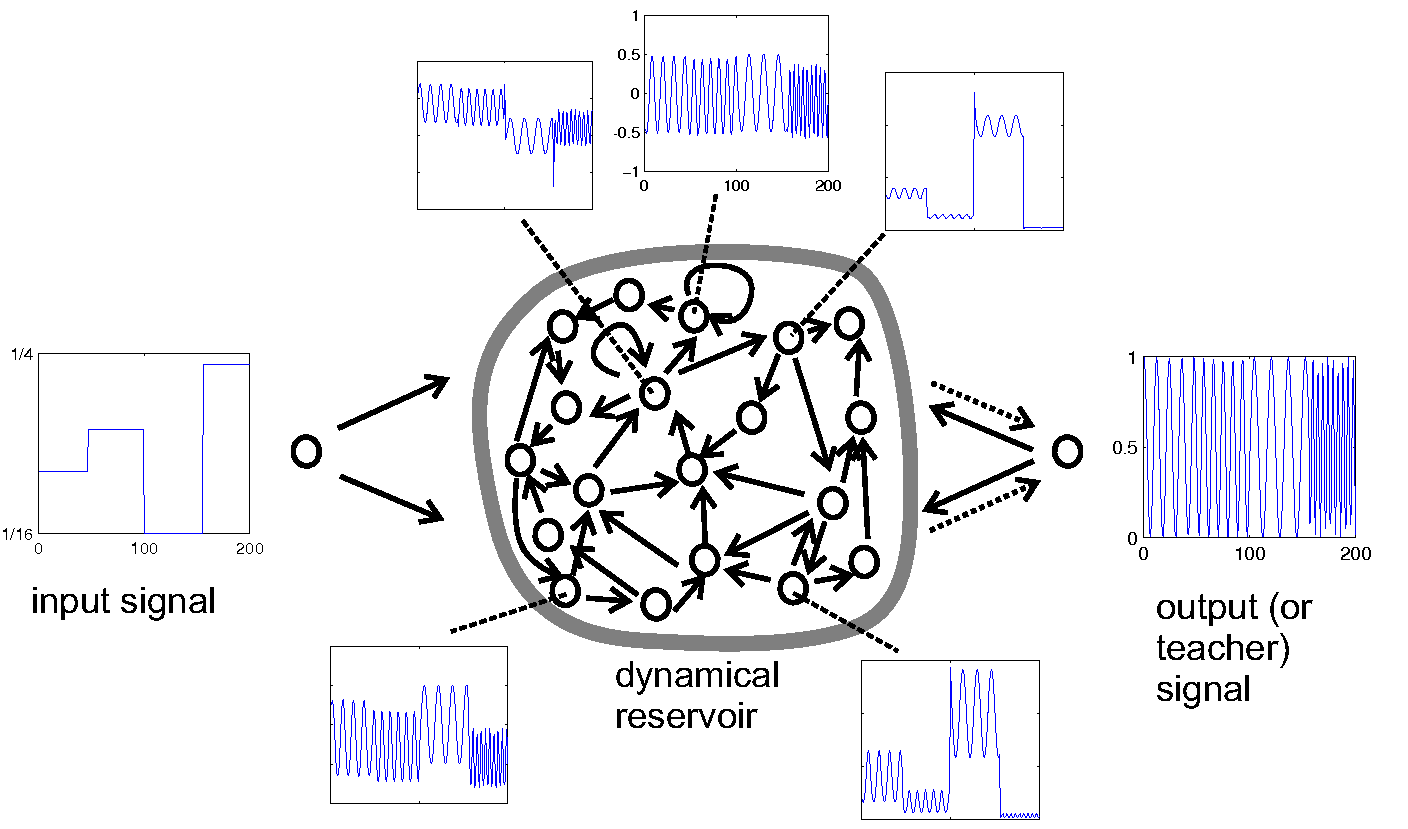
\includegraphics[width=\linewidth]{ESN_diag_FreqGenSchema.png}
                % \caption{ESN Diagram \cite{wiki:esn}} % Caption might clutter slide
            \end{figure}

        \column{0.5\textwidth}
            \textbf{Liquid State Machines (LSMs)} \cite{article_lsm_intro}
            \begin{itemize}
                \item Spiking neuron models
                \item Biologically inspired
                \item Computational neuroscience
            \end{itemize}
             \begin{figure}
                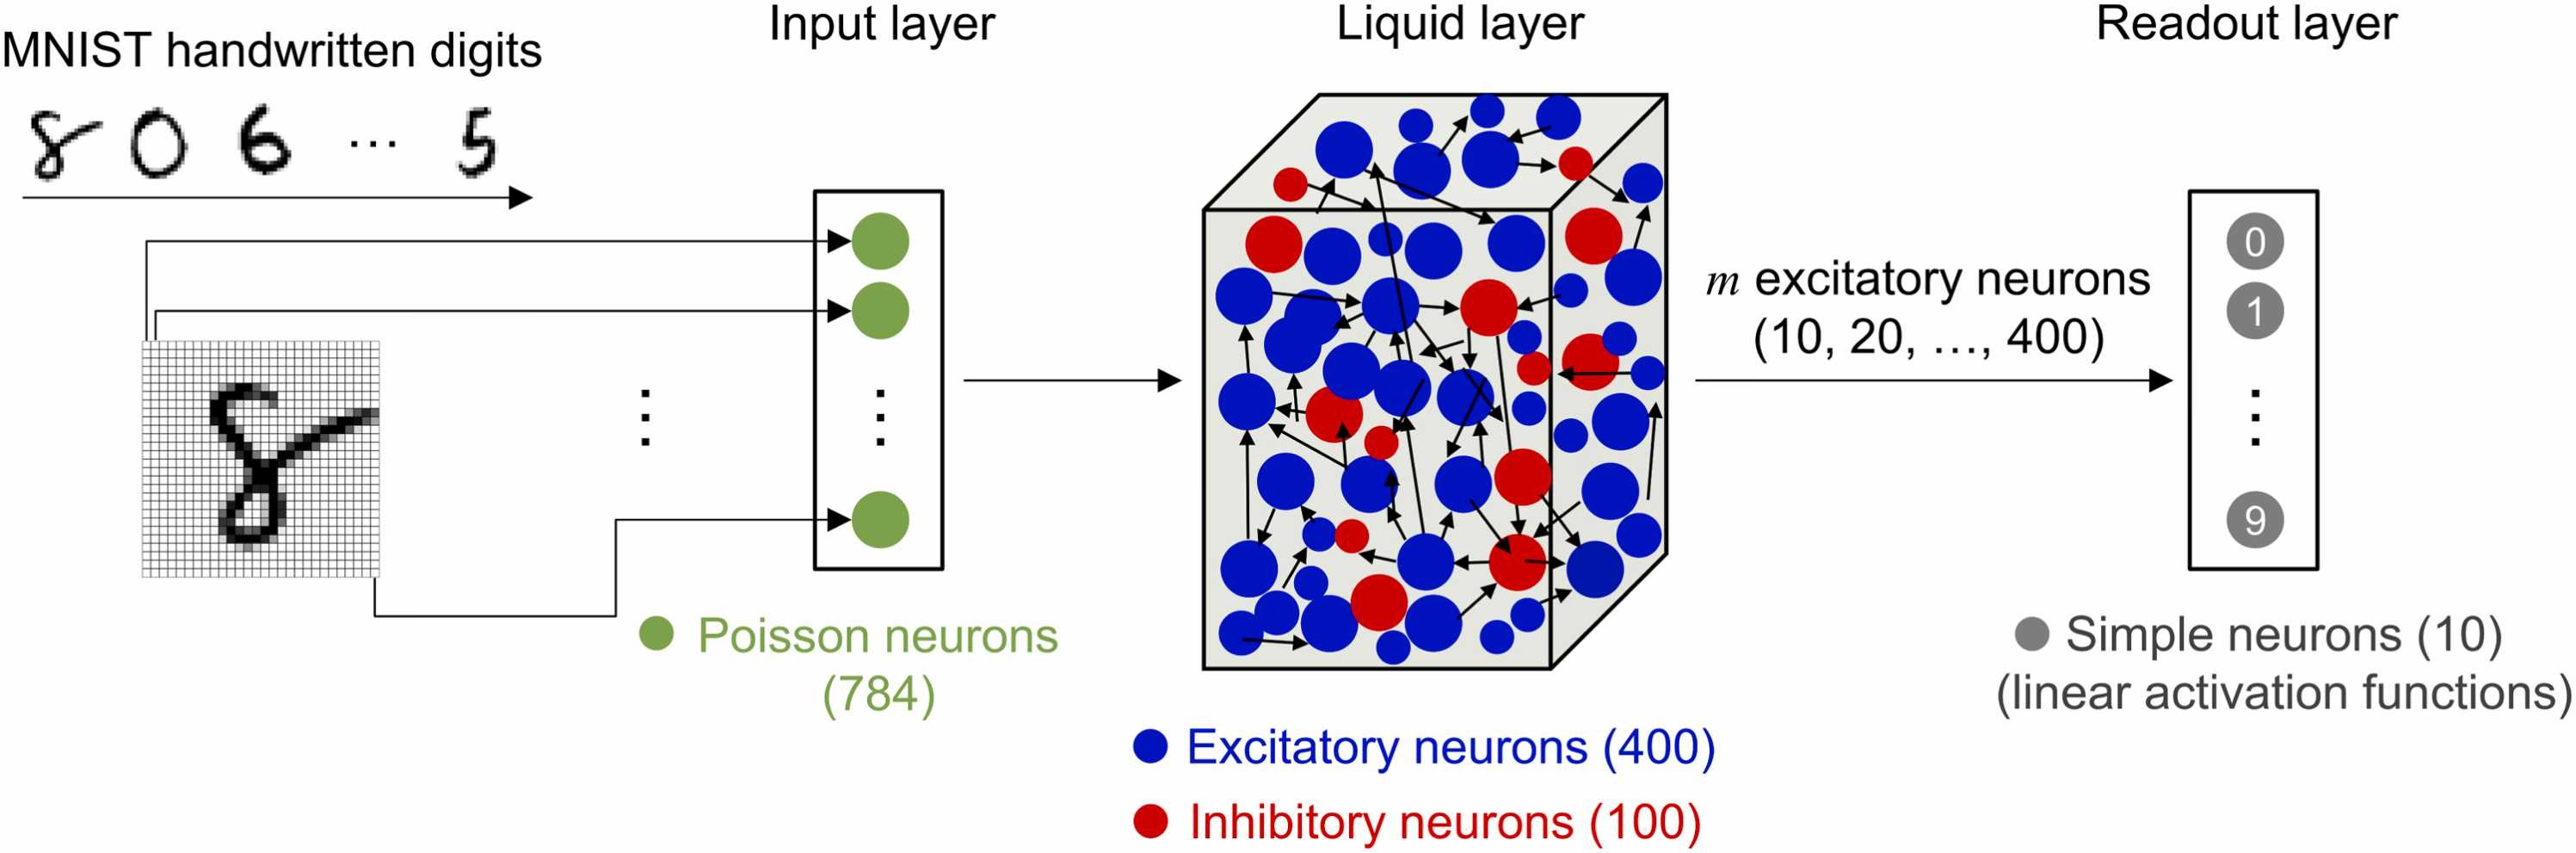
\includegraphics[width=\linewidth]{lsm_diag.png}
                 % \caption{LSM Diagram \cite{WOO2024129334}}
            \end{figure}
    \end{columns}
    \vspace{1em}
    \textbf{Physical Reservoir Computing (PRC):} Implements reservoirs using physical systems (optics, mechanics, etc.) \cite{Mandal2022}.
\end{frame}

\begin{frame}
    \frametitle{Training Methodology}
    Remarkably simple compared to RNNs:
    \begin{enumerate}
        \item \textbf{Collect States:} Feed input signals $\mathbf{u}$ into the fixed reservoir and record the sequence of reservoir states $\mathbf{x}$. Store states in a matrix $G$.
        \item \textbf{Collect Targets:} Obtain the corresponding target output sequence $Y$.
        \item \textbf{Train Readout:} Solve for the output weights $\mathbf{W}^{\mathrm{out}}$ using linear regression (often Ridge Regression to prevent overfitting).
    \end{enumerate}
    \pause
    \textbf{Ridge Regression Formulation:}
    \[
    W_{\text{out}} = YG^T\left(GG^T + \lambda I\right)^{-1}
    \]
    \begin{itemize}
        \item $G$: Matrix of collected reservoir states (each column is a state $\mathbf{x}[n]$)
        \item $Y$: Matrix of target outputs
        \item $\lambda$: Regularization parameter
        \item $I$: Identity matrix
    \end{itemize}
    \pause
    \begin{enumerate}
        \setcounter{enumi}{3}
        \item \textbf{Inference:} Apply the trained $W_{\text{out}}$ to new reservoir states generated from unseen inputs.
    \end{enumerate}
\end{frame}

\begin{frame}
    \frametitle{Advantages and Limitations}
    \textbf{Advantages:}
    \begin{itemize}
        \item [+] Fast, simple training (linear regression)
        \item [+] Avoids gradient problems of RNNs
        \item [+] Same reservoir can be used for multiple tasks (train different readouts)
        \item [+] Suitable for physical implementations (fixed reservoir)
        \item [+] Good at capturing temporal dynamics with low overhead
    \end{itemize}
    \pause
    \textbf{Limitations:}
    \begin{itemize}
        \item [-] Random initialization gives less control over function
        \item [-] Memory capacity limited by reservoir size
        \item [-] Performance depends on task/reservoir match \cite{article_RC_intro}
        \item [-] Sensitive to hyperparameter tuning (spectral radius, size, leak rate, etc.)
        \item [-] May struggle with tasks requiring very long memory or complex state representations compared to trained RNNs \cite{article_catch_22s_rc}
    \end{itemize}
\end{frame}

% --- Section 3: Literature Review Highlights ---
\section{Literature Review Highlights}

\begin{frame}
    \frametitle{Key Ideas from Literature}
    \begin{itemize}
        \item \textbf{\cite{article_RC_intro}:} Foundational tutorial on setting up RC experiments.
        \pause
        \item \textbf{\cite{article_catch_22s_rc}:} Explored RC limitations ("Catch-22s"), especially for complex tasks like basin prediction; requires long warm-up or precise system knowledge (NGRC).
        \pause
        \item \textbf{\cite{Arun2024}:} Demonstrated simple discrete maps (like logistic map with virtual nodes) can act as effective reservoirs, even with noise.
        \pause
        \item \textbf{\cite{Mandal2022}:} Showed even a minimal physical system (single driven pendulum) can perform RC tasks by exploiting transient dynamics.
        \pause
        \item \textbf{\cite{Itoh2020}:} Successfully reconstructed bifurcation diagrams from noisy time-series using ELM (a type of RC readout) combined with PCA, demonstrating inference of global dynamics.
    \end{itemize}
\end{frame}

% --- Section 4: Implementation and Results ---
\section{Implementation and Results}

% --- Subsection 4.1: Pendulum Reservoir ---
\subsection{Pendulum Reservoir}

\begin{frame}
    \frametitle{Experiment 1: Pendulum as Reservoir}
    \textbf{Goal:} Replicate \cite{Mandal2022} - use a single physical oscillator.
    \vspace{1em}
    \textbf{System: Driven Damped Pendulum}
    \begin{equation*} % No label needed
    \begin{aligned}
    \frac{dx}{dt} &= v \\
    \frac{dv}{dt} &= -\frac{g}{l} \sin(x) - k v + f \, \text{sign}(\sin(\omega t))
    \end{aligned}
    % \label{eq:pendulum_slide} % No label needed
    \end{equation*}
    \begin{itemize}
        \item Input signal $\mathbf{u}(t)$ injected as driving force $f$.
        \item Reservoir state $\mathbf{x}(t)$ is $[x(t), v(t)]$ (angle, velocity).
        \item Exploit rich transient dynamics.
    \end{itemize}
    \pause
    \textbf{Task:} Predict a target time series (e.g., delayed input).
    \vspace{1em}
    Train linear readout $W_{\text{out}}$ on collected states $[x(t_i), v(t_i)]$.
\end{frame}

\begin{frame}
    \frametitle{Pendulum Reservoir: Simple Prediction Result}
     \begin{figure}
        \centering
        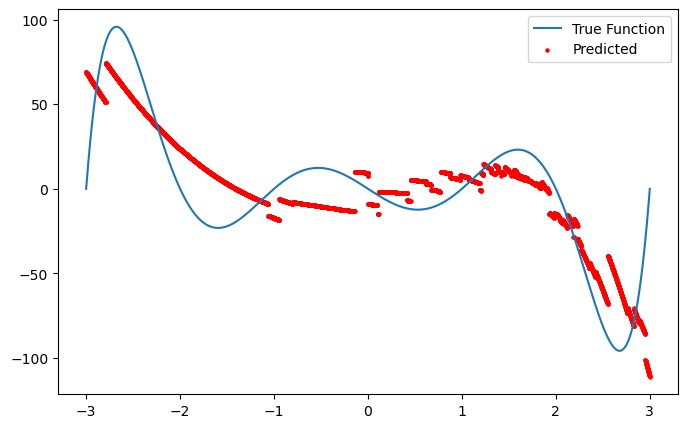
\includegraphics[width=0.75\linewidth]{pendulum_result_0.png}
        \caption{Predicting a target function using pendulum states (driven by $x_{t-1}$). Shows learning capability, though hyperparameters matter.}
        \label{fig:pendulum-1_slide}
    \end{figure}
    \textit{Demonstrates that even a simple oscillator can function as a reservoir.}
\end{frame}

\begin{frame}
    \frametitle{Pendulum Reservoir: Lorenz System Prediction}
    \textbf{Task:} Predict the full state $(x, y, z)$ of the Lorenz system given only the $x(t)$ component as input to the pendulum reservoir.
    \vspace{1em}
    \textbf{Lorenz System ($\sigma=10, \rho=28, \beta=8/3$):}
    \begin{equation*} % No label needed
    \begin{aligned}
    \frac{dx}{dt} &= \sigma (y - x) \\
    \frac{dy}{dt} &= x (\rho - z) - y \\
    \frac{dz}{dt} &= x y - \beta z
    \end{aligned}
    \end{equation*}
    \pause
     \begin{figure}
        \centering
        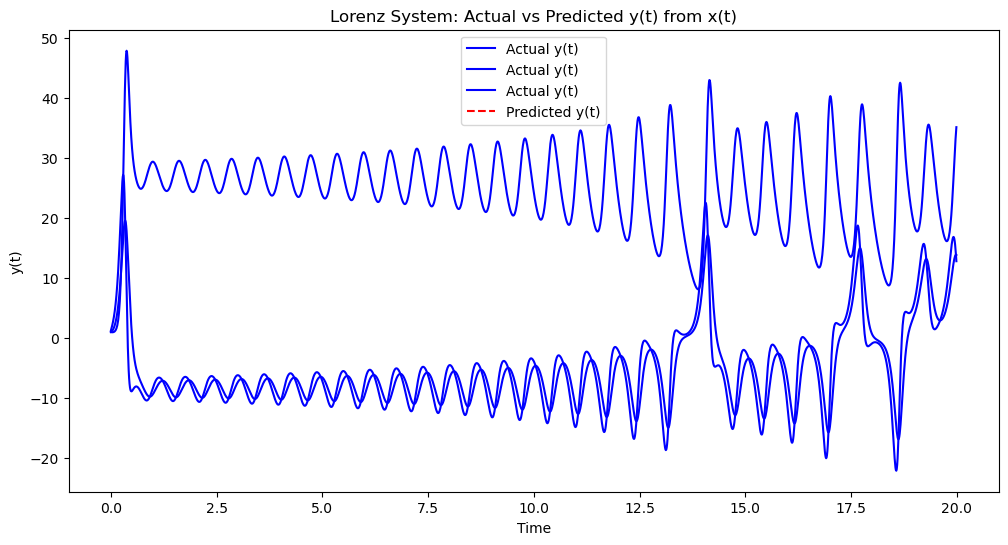
\includegraphics[width=1\linewidth]{lorentz_pendulum_1.png}
        \caption{Actual vs. Predicted $y(t)$ for Lorenz system using Pendulum reservoir (input $x(t)$ only).}
        \label{fig:lorentz_1_slide}
    \end{figure}
\end{frame}

\begin{frame}
    \frametitle{Pendulum Reservoir: Lorenz Attractor}
     \begin{figure}
        \centering
        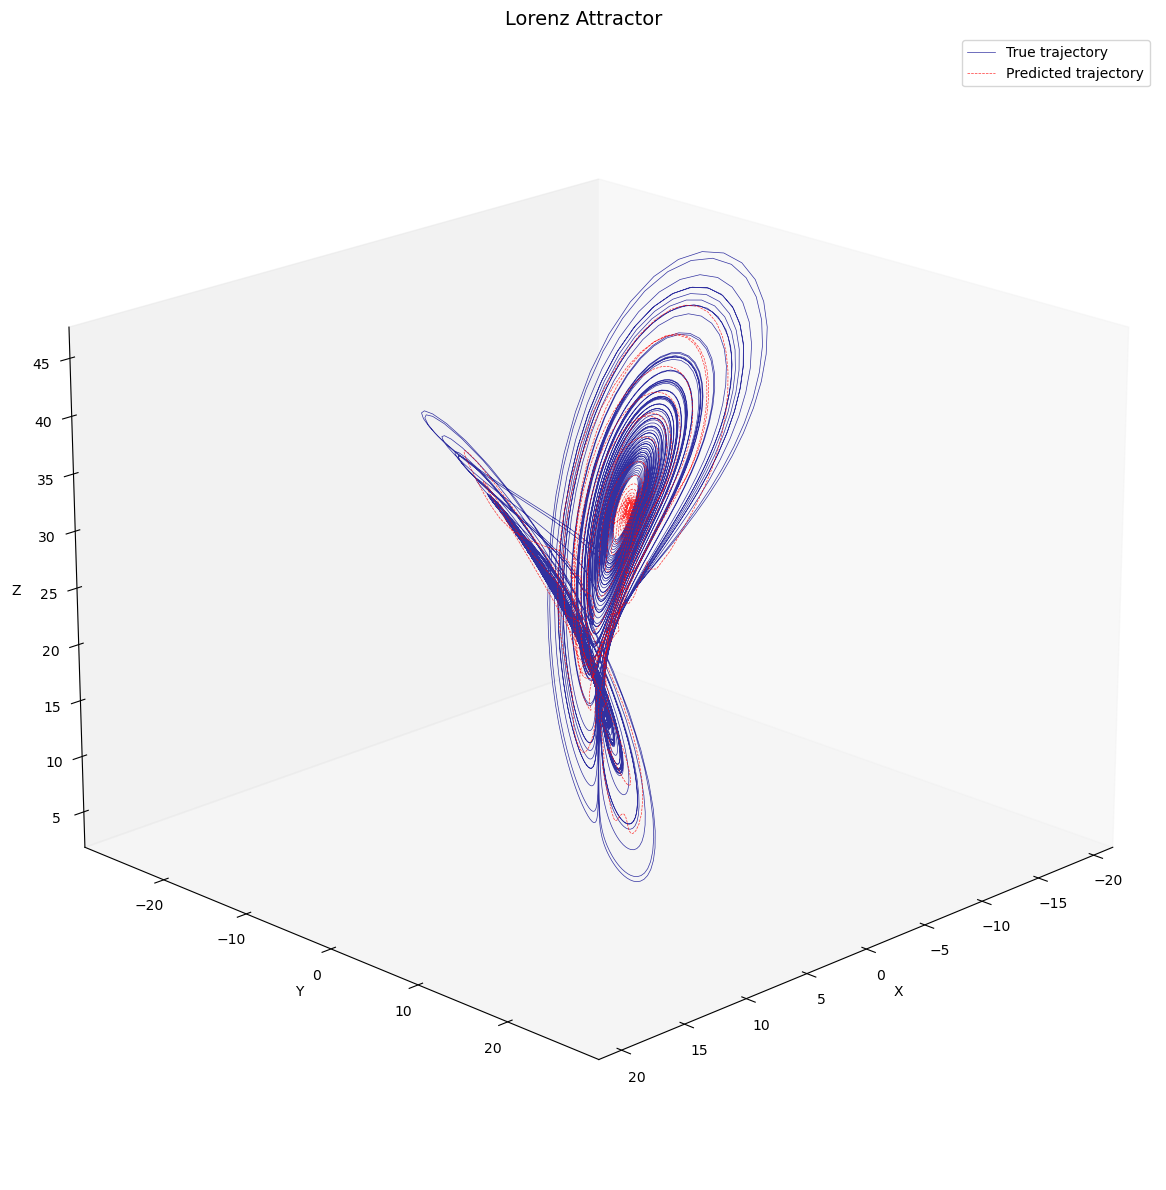
\includegraphics[width=0.9\linewidth]{lorentz_pendulum_2.png}
        \caption{3D view of the Lorenz attractor: True (blue) vs. Predicted (red) using the pendulum reservoir.}
        \label{fig:lorentz_2_slide}
    \end{figure}
    \textit{Captures the overall structure but with deviations.}
\end{frame}

% --- Subsection 4.2: Logistic Map Reservoir ---
\subsection{Logistic Map Reservoir}

\begin{frame}
    \frametitle{Experiment 2: Logistic Map as Reservoir}
    \textbf{Goal:} Replicate \cite{Arun2024} - use a discrete map with virtual nodes.
    \vspace{1em}
    \textbf{System: Logistic Map}
    \[ x_{n+1} = r x_n (1 - x_n) \]
    \textbf{Reservoir Construction (Virtual Nodes):}
    \begin{itemize}
        \item For each input $u_n$, iterate the map multiple times.
        \item Sample intermediate states $x_{n,k}$.
        \item Combine samples (e.g., with trigonometric functions) to form high-dimensional state vector $\mathbf{x}[n]$.
    \end{itemize}
    \pause
    \textbf{Task 1: Benchmark - 7th Degree Polynomial}
     \begin{figure}
        \centering
        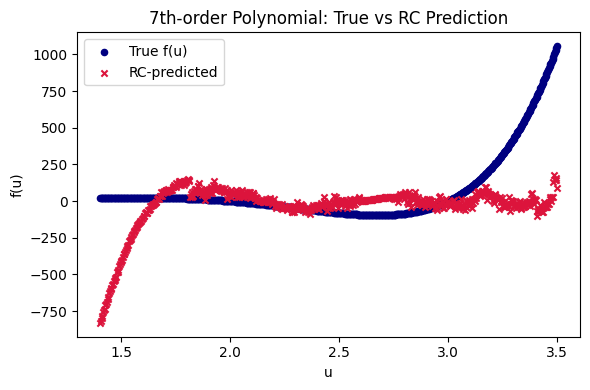
\includegraphics[width=0.75\linewidth]{logistic_7th_degree.png}
        \caption{Predicting a polynomial using the logistic map reservoir. Shows effectiveness for non-temporal tasks too.}
        \label{fig:logistic_map_slide}
    \end{figure}
\end{frame}

\begin{frame}
    \frametitle{Logistic Map Reservoir: Lorenz System Prediction}
    \textbf{Task 2:} Predict Lorenz system state $(x, y, z)$ given $x(t)$ as input.
    \vspace{1em}
    \textbf{Result (RMSE):} [x: 3.77, y: 2.94, z: 8.36] - Reasonable accuracy.
    \pause
     \begin{figure}
        \centering
        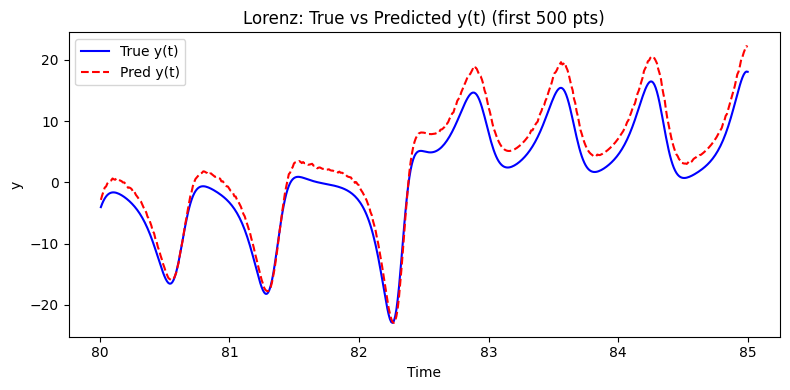
\includegraphics[width=1\linewidth]{lorentz_logistic_pred_true.png}
        \caption{Actual vs. Predicted $y(t)$ for Lorenz system using Logistic Map reservoir.}
        \label{fig:logistic_map_lorenz_slide}
    \end{figure}
\end{frame}

\begin{frame}
    \frametitle{Logistic Map Reservoir: Lorenz Attractor Projections}
     \begin{figure}
        \centering
        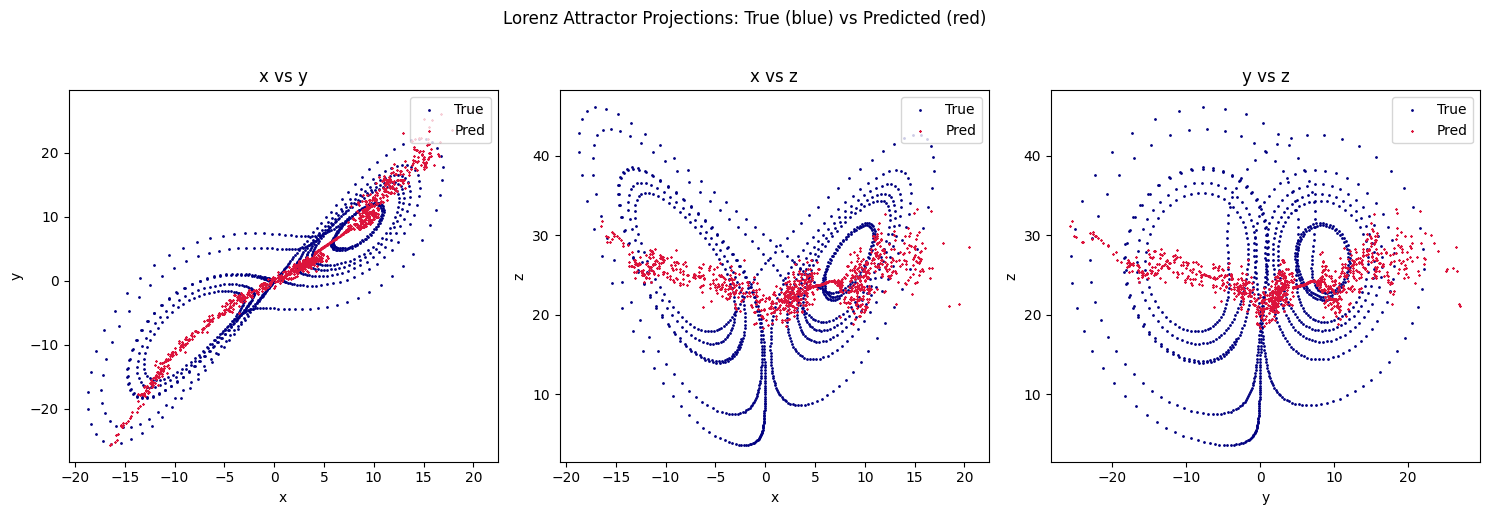
\includegraphics[width=1\linewidth]{lorenz_logistic_pred_diagram.png}
        \caption{Phase space projections: True (blue) vs. Predicted (red) using logistic map reservoir. Captures attractor shape well.}
        \label{fig:logistic_map_lorenz_diag_slide}
    \end{figure}
\end{frame}

% --- Subsection 4.3: Bifurcation Reconstruction (RC) ---
\subsection{Bifurcation Reconstruction via PCA + ELM}

\begin{frame}
    \frametitle{Experiment 3: Bifurcation Reconstruction (RC approach)}
    \textbf{Goal:} Replicate \cite{Itoh2020} - reconstruct dynamics from time series data across varying parameters. Use Logistic Map data as example.
    \vspace{1em}
    \textbf{Methodology:}
    \begin{enumerate}
        \item Generate time series $x_t$ for various parameter values $\mu$ (e.g., $r$ in logistic map). Add noise.
        \item Feed each time series through a reservoir (e.g., logistic map reservoir). Collect states $G_\mu$.
        \item Apply PCA to reservoir states $G_\mu$ to get low-dimensional features $P_\mu$.
        \item Train an ELM (Extreme Learning Machine - essentially an RC readout) to predict $x_{t+1}$ from $(P_{\mu, t}, \mu)$.
        \item Sweep $\mu$ and use the trained ELM to predict attractor points $\rightarrow$ Reconstruct Bifurcation Diagram.
    \end{enumerate}
\end{frame}

\begin{frame}
    \frametitle{Bifurcation Reconstruction (RC): First Attempt}
     \begin{figure}
        \centering
        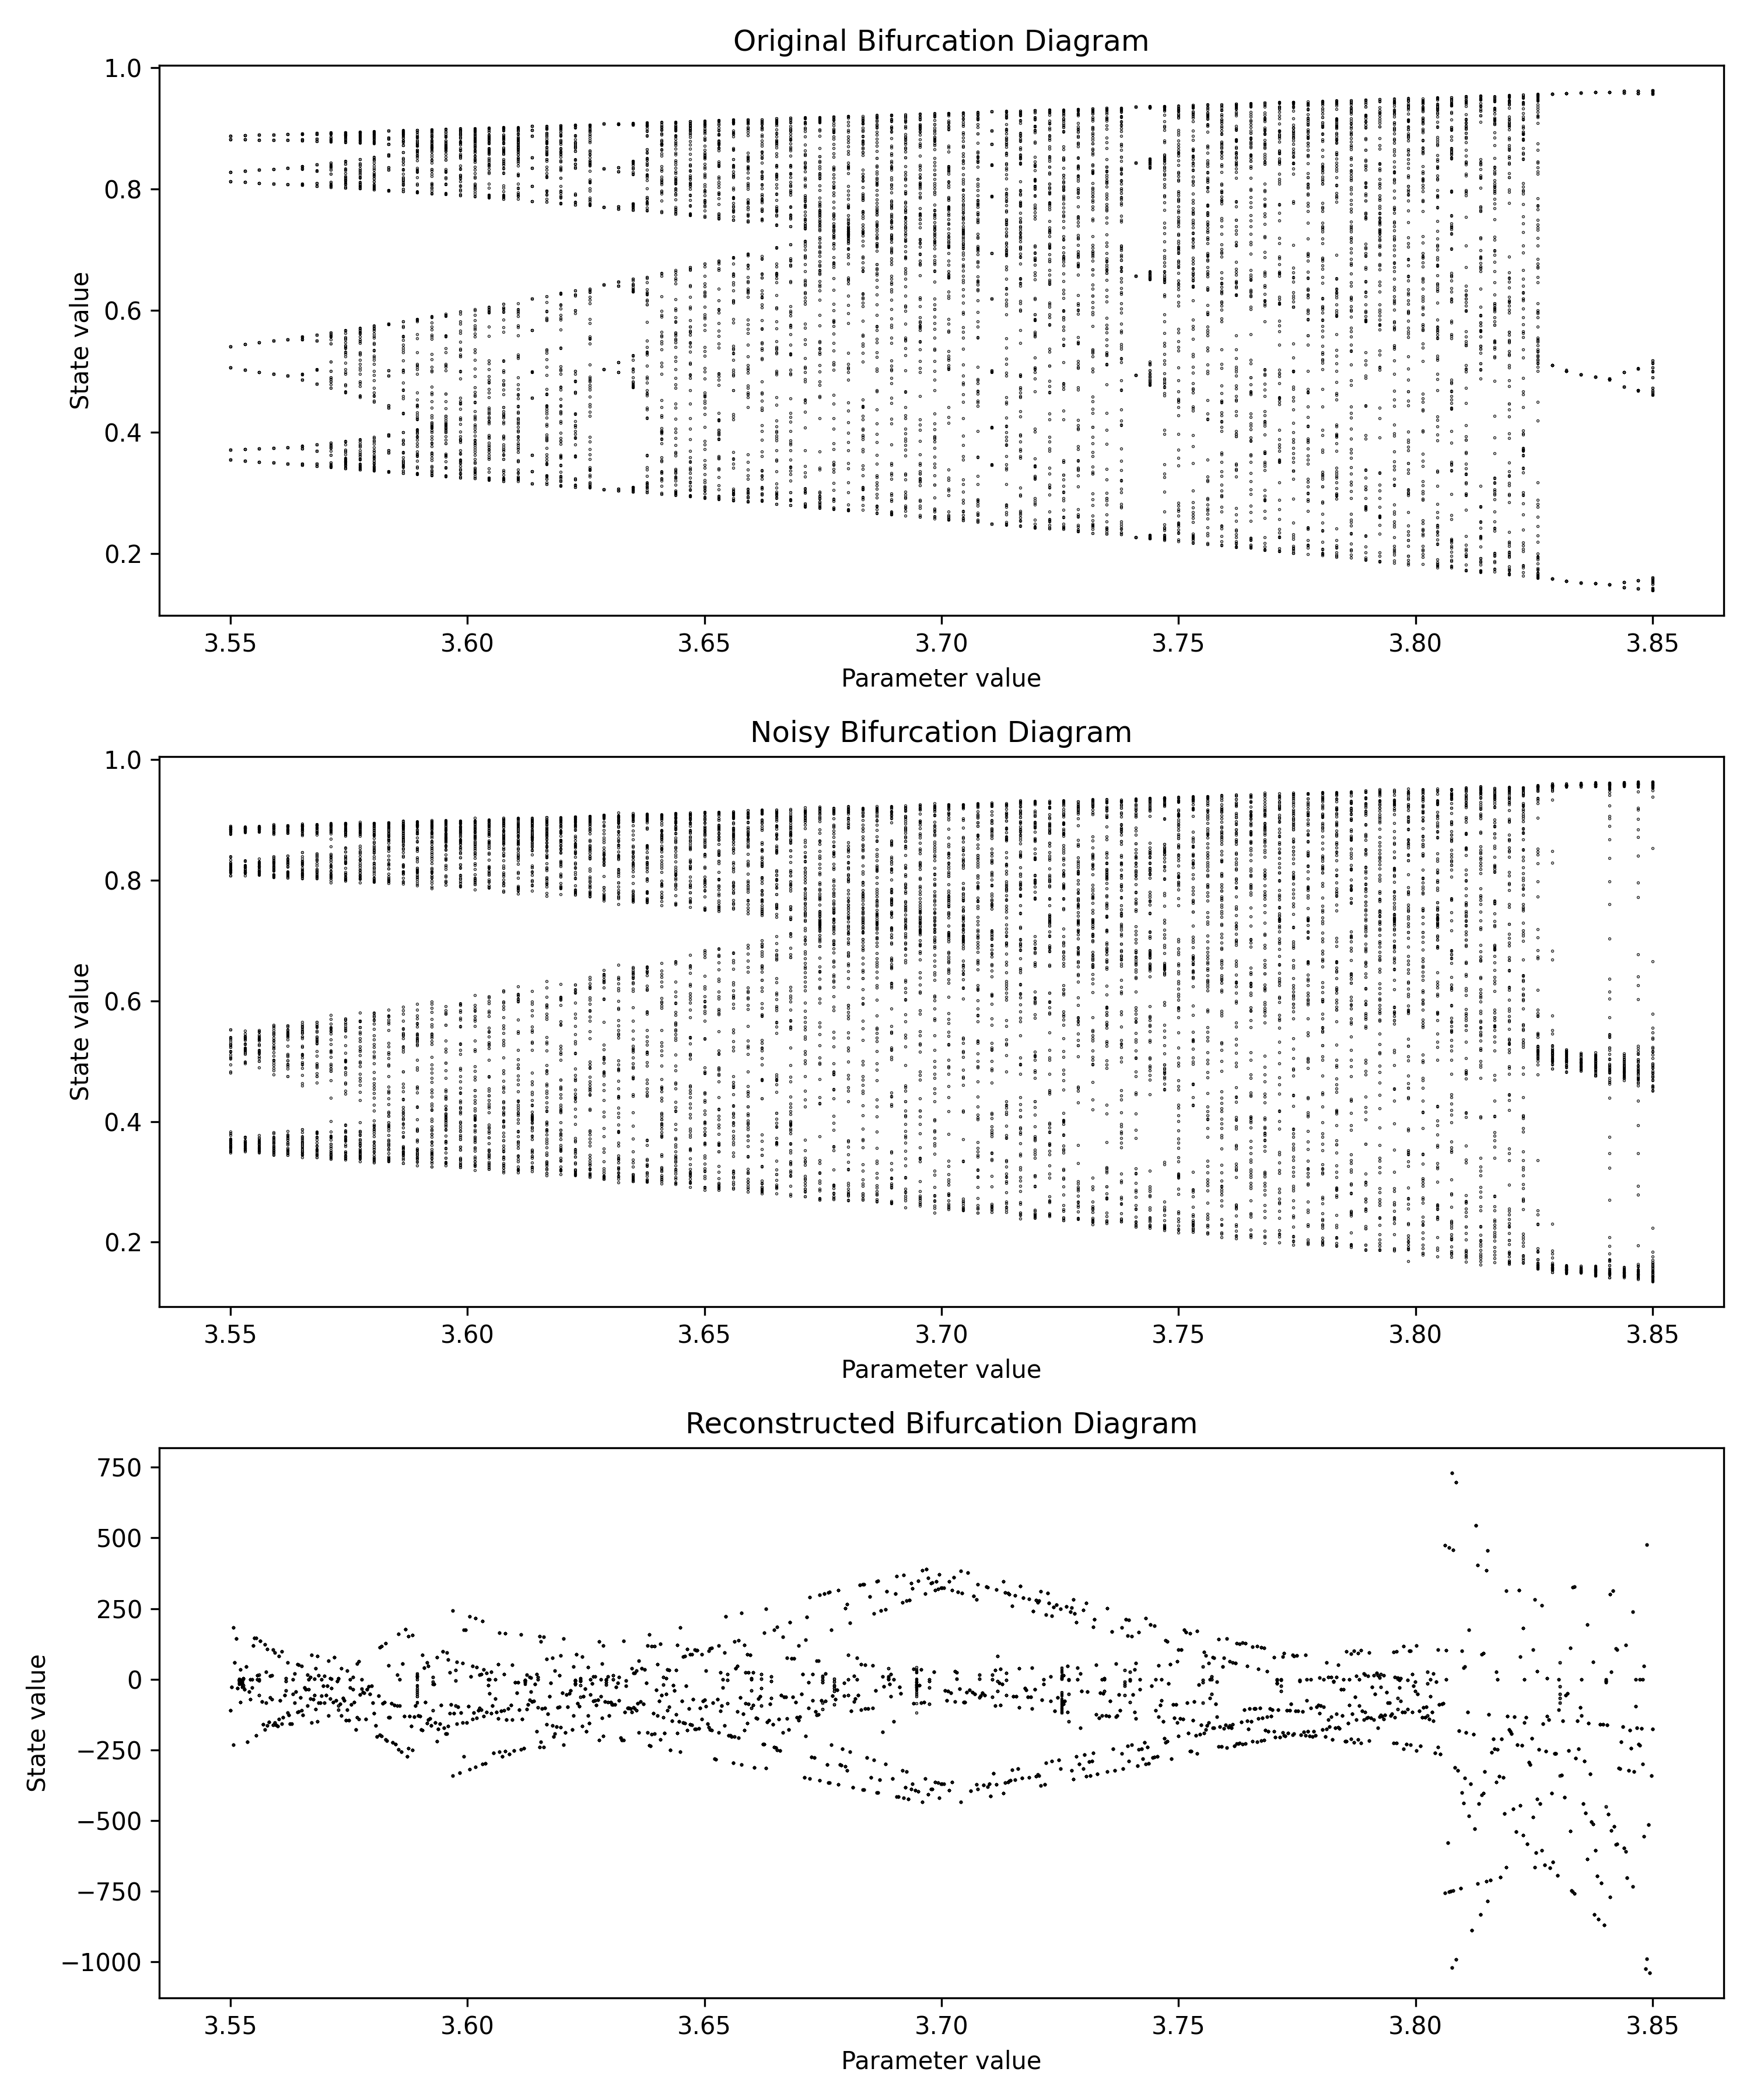
\includegraphics[width=1\linewidth]{bd_reconstruction_elm.png}
        \caption{Initial attempt: Original vs. Noisy vs. Reconstructed BD. Reconstruction is poor - missing branches, distorted.}
        \label{fig:bifurcation_slide}
    \end{figure}
    \textbf{Issues:} Sensitivity to noise, hyperparameters, potentially insufficient reservoir complexity or flawed implementation details (paper lacked specifics).
\end{frame}

\begin{frame}
    \frametitle{Bifurcation Reconstruction (RC): Improved Results}
     \begin{figure}
        \centering
        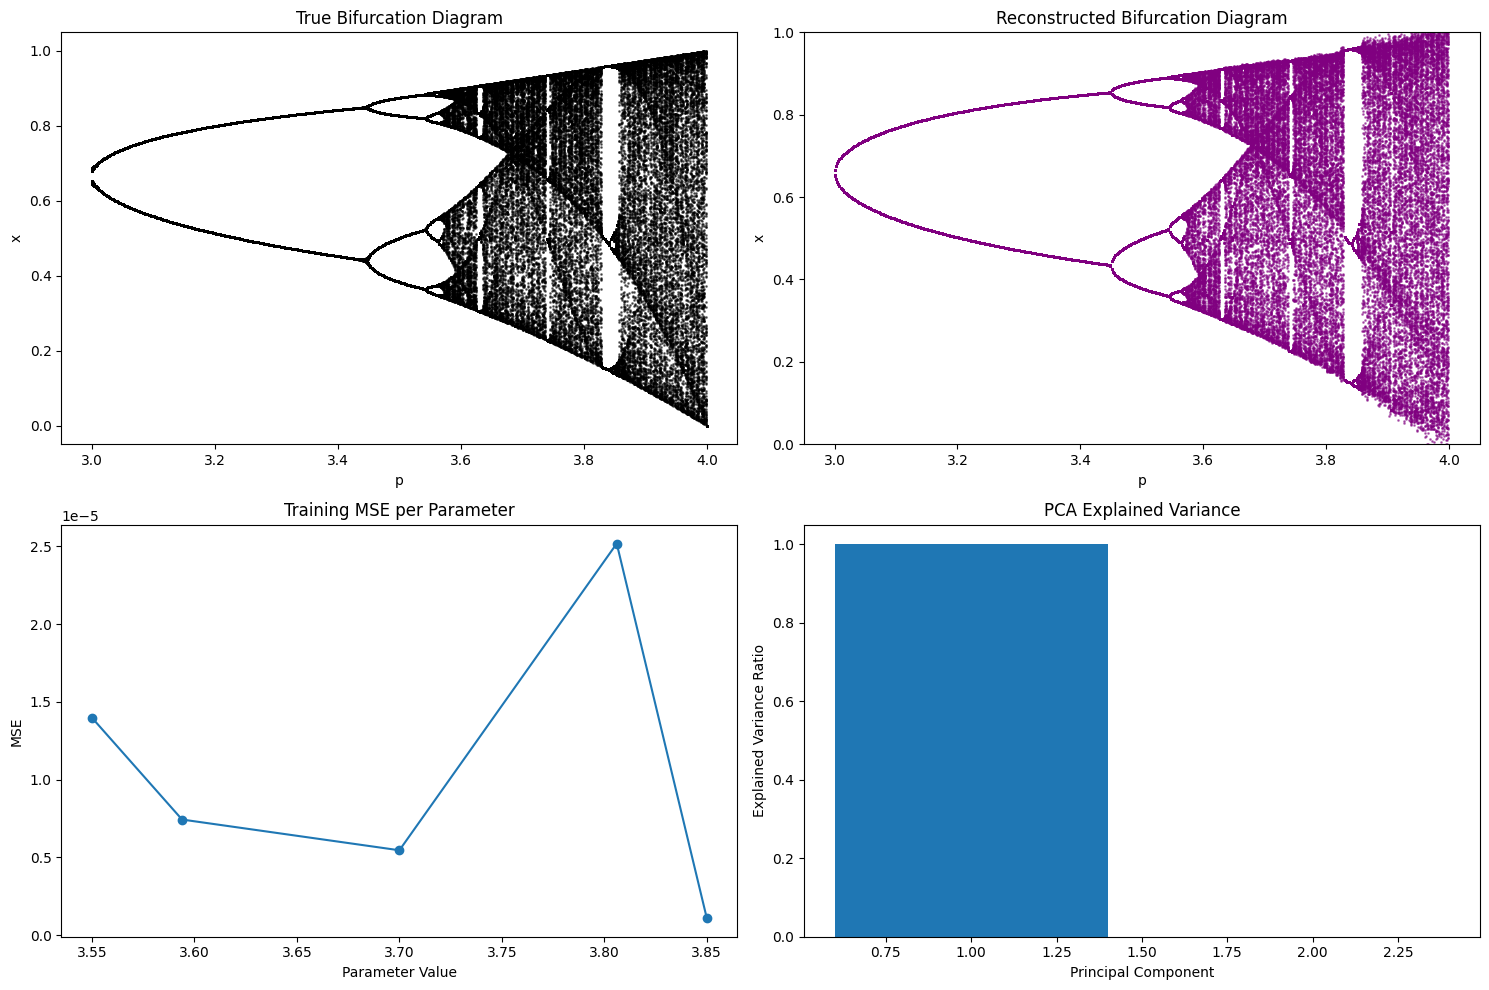
\includegraphics[width=1\linewidth]{bd_1_results.png}
        \caption{Improved Reconstruction (after tuning/fixes): Training MSE $\approx 10^{-5}$. Captures main period-doubling features. PCA shows variance explained.}
        \label{fig:bd_1_slide}
    \end{figure}
\end{frame}

\begin{frame}
    \frametitle{Bifurcation Reconstruction (RC): Return Maps}
     \begin{figure}
        \centering
        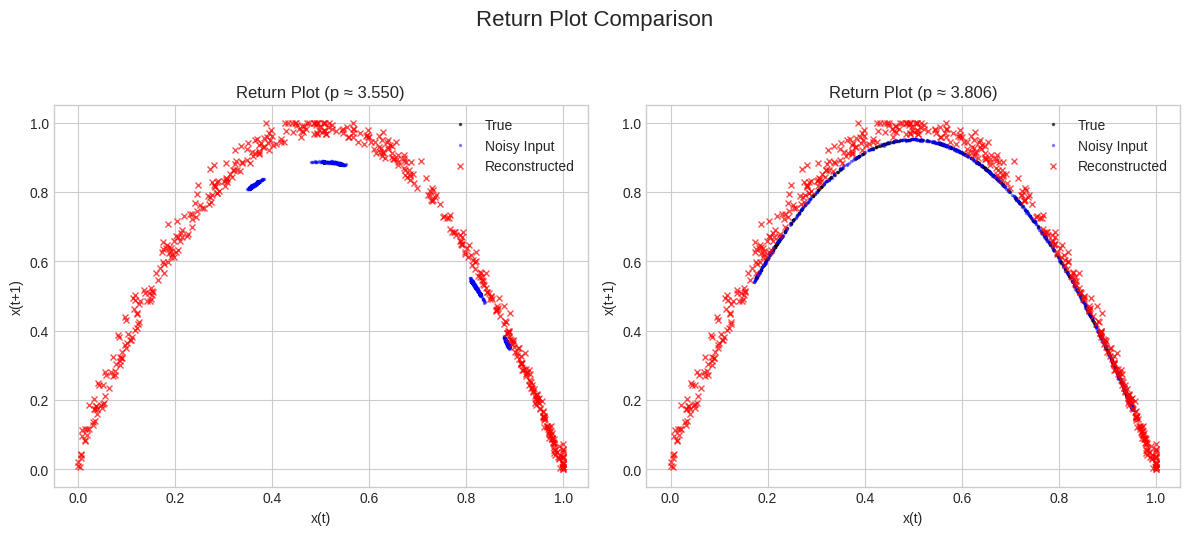
\includegraphics[width=1\linewidth]{bd_return_plot_2.png}
        \caption{Reconstructed return maps ($x_{t+1}$ vs $x_t$) for different parameter values (p=3.550, p=3.806). Matches noisy input structure well.}
        \label{fig:bd_2_slide}
    \end{figure}
\end{frame}


\begin{frame}
    \frametitle{Bifurcation Reconstruction (RC): Extrapolation Issue}
     \begin{figure}
        \centering
        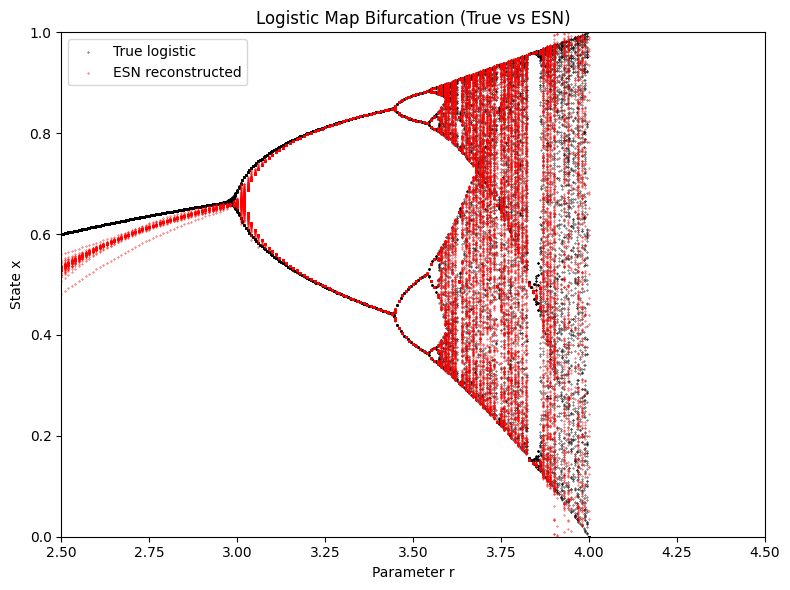
\includegraphics[width=0.8\linewidth]{bf_3_results_overlapped.png}
        \caption{Overlapped True (black) vs. Reconstructed (red) BDs. Good match within training range, but poor extrapolation outside.}
        \label{fig:bd_3_slide}
    \end{figure}
    \textit{RC struggles to generalize dynamics beyond the parameter range it was trained on.}
\end{frame}

\begin{frame}
    \frametitle{Bifurcation Reconstruction (RC): Lyapunov Exponents}
     \begin{figure}
        \centering
        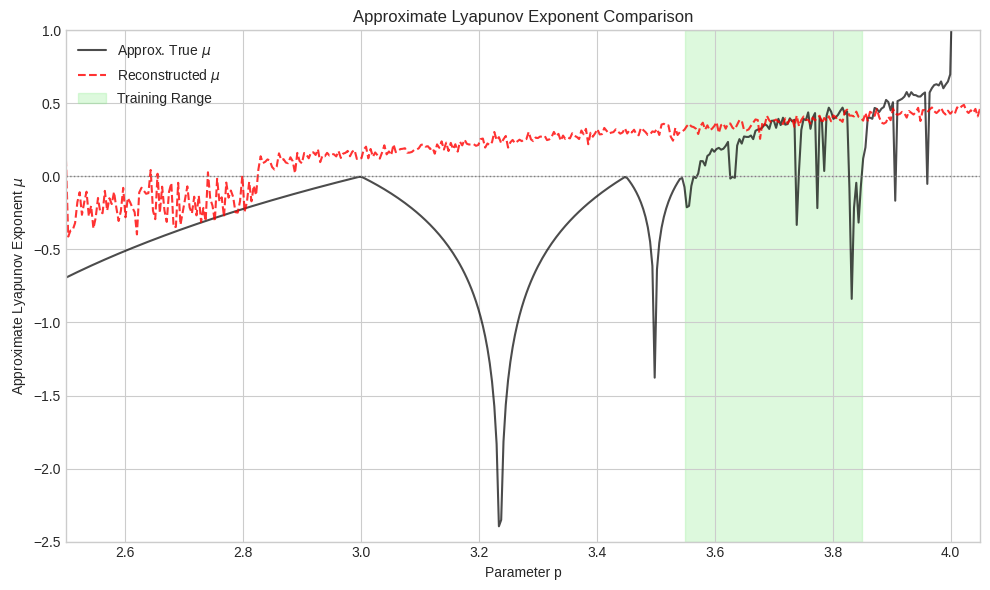
\includegraphics[width=1\linewidth]{lyapanov_bd_rd.png}
        \caption{Estimated Lyapunov exponents. Red line (reconstructed) approximates true exponent (black) within the training range (green shaded area), but diverges outside.}
        \label{fig:lypanov_bd_rc_slide}
    \end{figure}
\end{frame}

\begin{frame}
    \frametitle{Bifurcation Reconstruction (RC): PCA Analysis}
     \begin{figure}
        \centering
        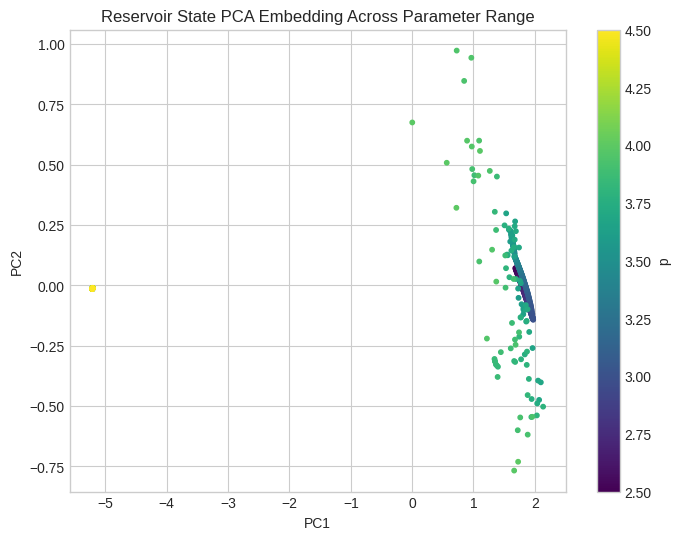
\includegraphics[width=0.8\linewidth]{bd_elm_pca_analysis.png}
        \caption{PCA embedding of reservoir states across parameter range. Shows how the reservoir state representation changes with the parameter $\mu$.}
        \label{fig:bd_4_slide}
    \end{figure}
\end{frame}


\begin{frame}
    \frametitle{Bifurcation Reconstruction (RC): Time Series Prediction}
     \begin{figure}
        \centering
        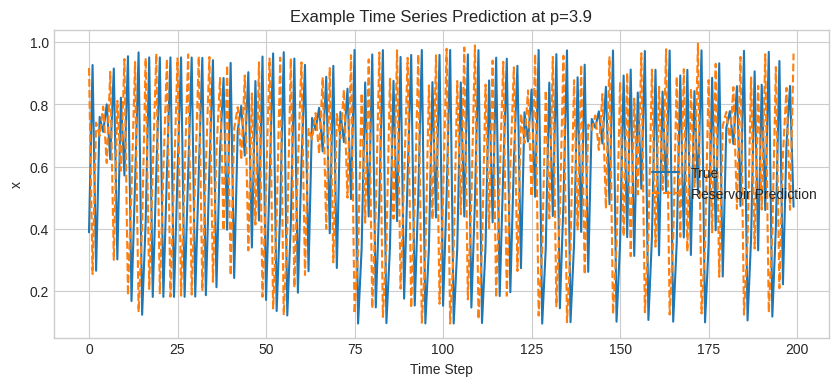
\includegraphics[width=1.0\linewidth]{bd_5_prediction_for_specific_value.png}
        \caption{Predicting time series evolution for a specific parameter value (p=3.9) using the trained ELM.}
        \label{fig:bd_5_slide}
    \end{figure}
\end{frame}

% --- Subsection 4.4: Bifurcation Reconstruction (LSTM) ---
\subsection{Using Recurrent Networks (LSTM) for Reconstruction}

\begin{frame}
    \frametitle{Experiment 4: Bifurcation Reconstruction (LSTM approach)}
    \textbf{Motivation:} The RC (ESN/ELM) approach struggled with accurate reconstruction, especially outside the training parameter range. The fixed reservoir couldn't easily adapt to parameter changes.
    \vspace{1em}
    \textbf{Alternative: Long Short-Term Memory (LSTM) Network}
    \begin{itemize}
        \item A type of RNN capable of learning long-range dependencies.
        \item All weights are trained end-to-end.
    \end{itemize}
    \begin{figure}
        \centering
        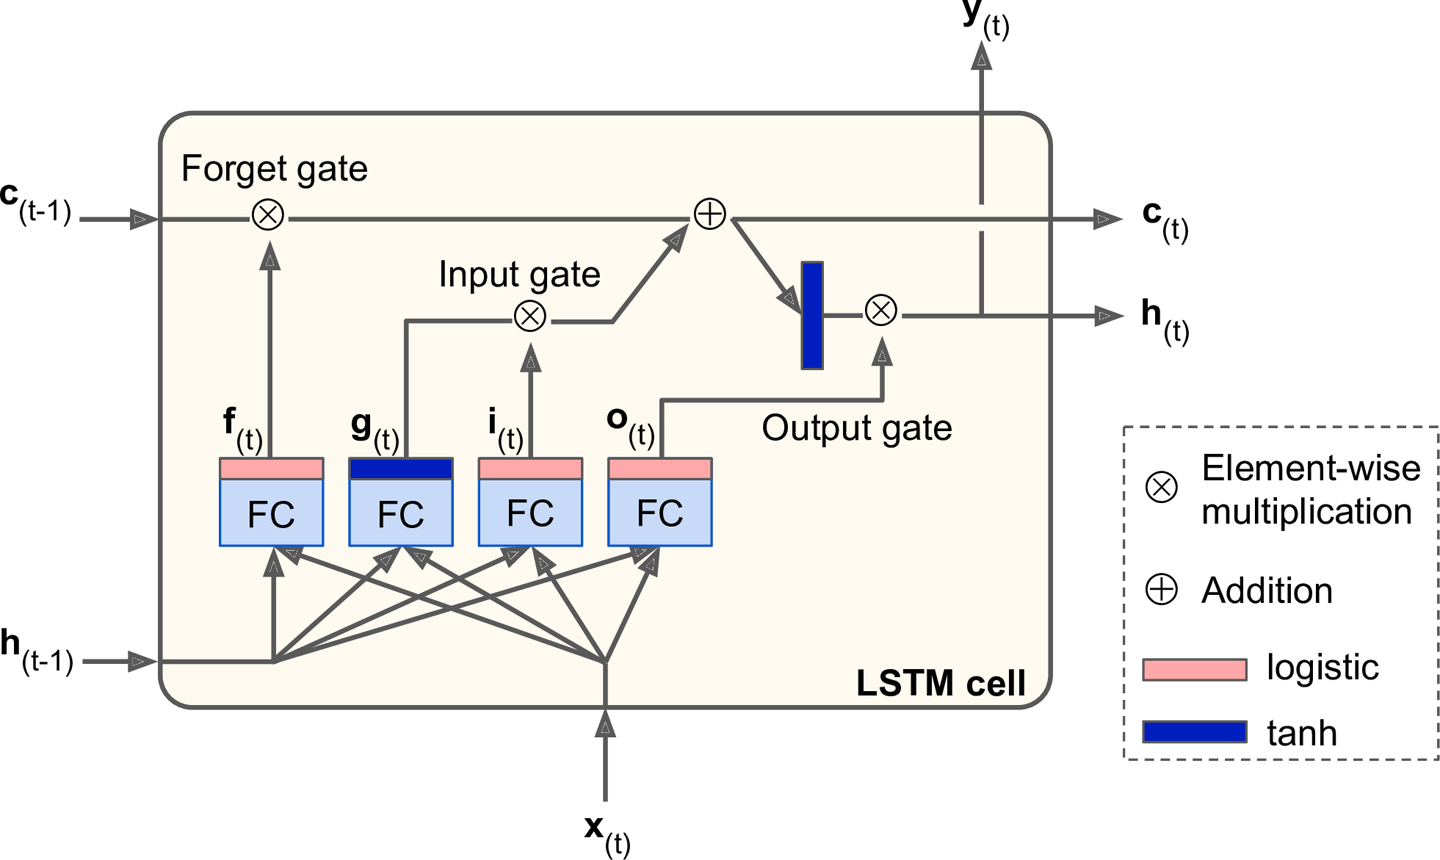
\includegraphics[width=0.8\linewidth]{LSTM_arch.png}
        \caption{Basic LSTM Cell Architecture.}
        \label{fig:lstm_arch_slide}
    \end{figure}
\end{frame}

\begin{frame}
    \frametitle{LSTM Approach: Key Differences}
    \begin{enumerate}
        \item \textbf{Parameter as Explicit Input:} LSTM learns a mapping $g_{\text{LSTM}}(x_t, p; \theta) \rightarrow \hat{x}_{t+1}$. The parameter $p$ is fed directly into the network.
        \pause
        \item \textbf{Learning Conditional Dynamics:} The network learns how dynamics change \textit{conditioned} on $p$ across the entire training dataset.
        \pause
        \item \textbf{End-to-End Training:} Internal recurrent dynamics adapt during training (via backpropagation) specifically for this task, unlike the fixed RC reservoir.
        \pause
        \item \textbf{Reconstruction via Iteration:} Iterate the trained LSTM: $\hat{x}_{t+1} = g_{\text{LSTM}}(\hat{x}_t, p^*; \theta)$ for any desired $p^*$.
    \end{enumerate}
    \vspace{1em}
    \textit{Hypothesis: Explicit parameter handling and trainable dynamics lead to better reconstruction.}
\end{frame}

\begin{frame}
    \frametitle{LSTM Reconstruction: Bifurcation Diagram}
    \begin{figure}
        \centering
        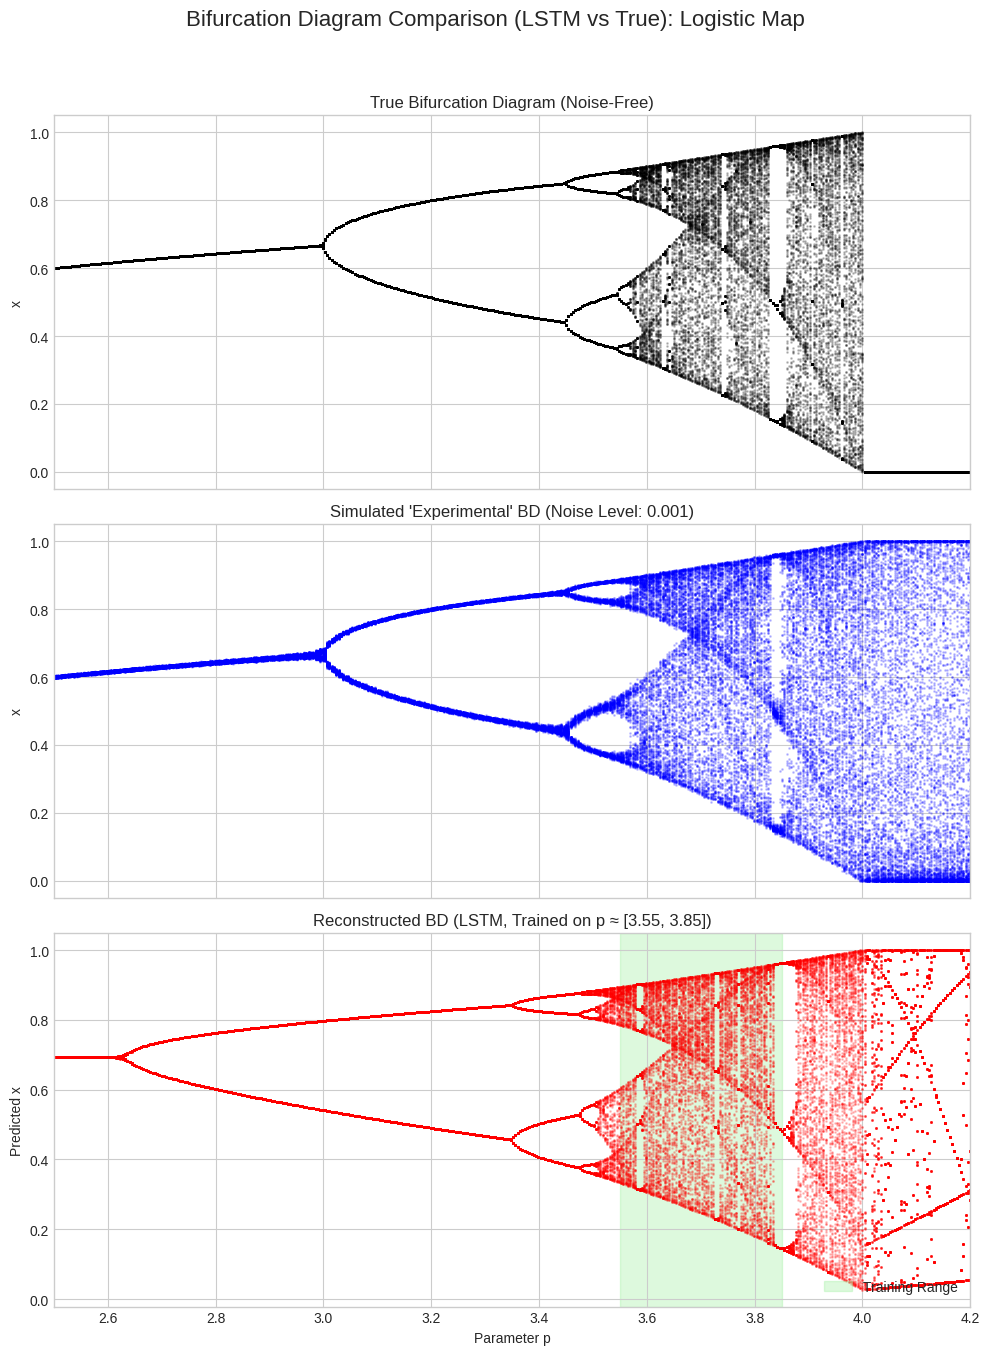
\includegraphics[width=1.0\linewidth]{lstm_bd_1.png}
        \caption{Comparison: True BD vs. Simulated Noisy BD vs. LSTM Reconstructed BD. LSTM (bottom) captures dynamics well, even slightly outside the training range (green area).}
        \label{fig:lstm_bd_1_slide}
    \end{figure}
\end{frame}

\begin{frame}
    \frametitle{LSTM Reconstruction: Return Maps}
    \begin{figure}
        \centering
        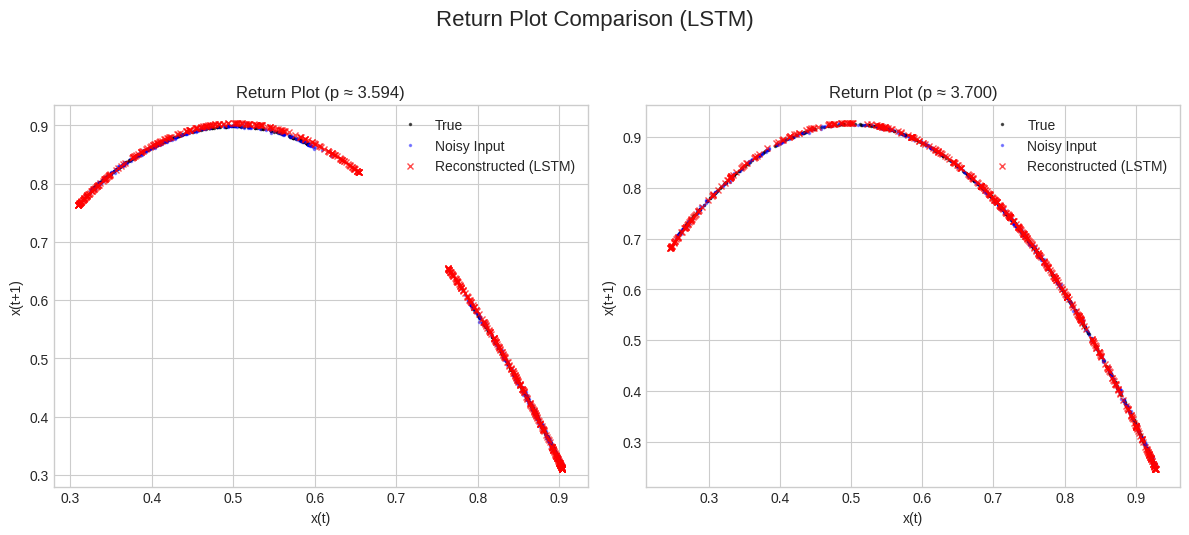
\includegraphics[width=1\linewidth]{lstm_bd_2.png}
        \caption{LSTM-reconstructed return maps for different parameter values. Accurately captures the underlying map shape.}
        \label{fig:lstm_bd_2_slide}
    \end{figure}
\end{frame}

\begin{frame}
    \frametitle{LSTM Reconstruction: Lyapunov Exponents}
    \begin{figure}
        \centering
        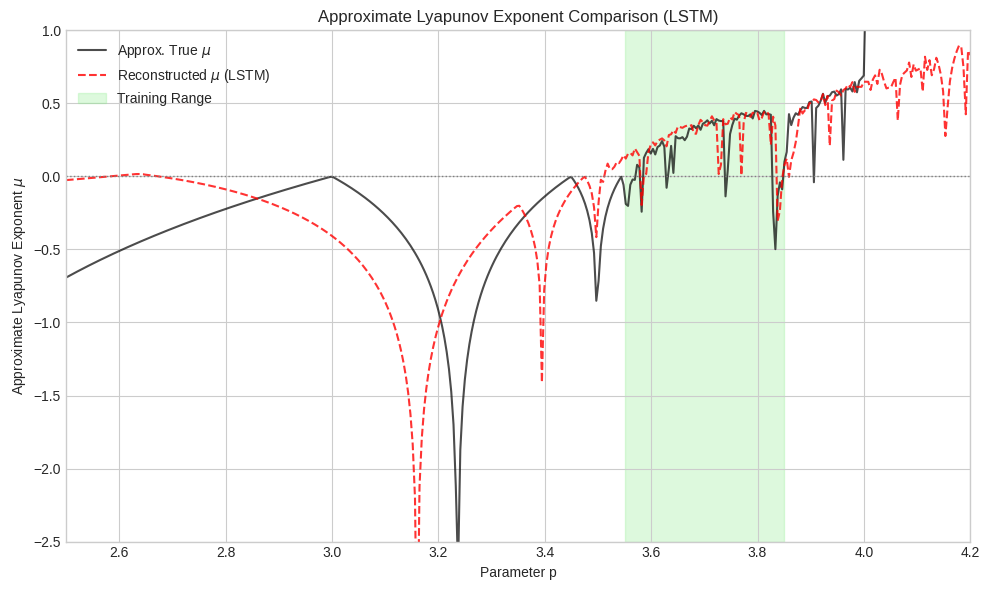
\includegraphics[width=1\linewidth]{lstm_bd_3.png}
        \caption{LSTM estimation of Lyapunov exponents. Shows better agreement with the true exponent (black) compared to the RC approach, especially in extrapolation.}
        \label{fig:lstm_bd_3_slide} % Note: label was enter-label in report
    \end{figure}
\end{frame}

\begin{frame}
    \frametitle{RC vs. LSTM: Training Time \& Compute}
    \textbf{Key Usability Difference:}
    \begin{itemize}
        \item \textbf{RC (ELM + PCA):} Training took \textbf{$<$ 1 second}.
            \begin{itemize}
                \item Advantage: Extremely fast training due to linear regression only.
            \end{itemize}
        \item \textbf{LSTM:} Training took \textbf{$\sim$ 46 seconds}.
            \begin{itemize}
                \item Disadvantage: Slower due to end-to-end backpropagation.
            \end{itemize}
    \end{itemize}
    \pause
    \textbf{Trade-off:}
    \begin{itemize}
        \item RC offers incredible speed, suitable for resource-constrained or real-time physical systems.
        \item LSTM (and other modern RNNs/Transformers/State Space Models \cite{gu2024mambalineartimesequencemodeling}) offers potentially higher accuracy and better generalization for complex tasks, especially when compute is less of a bottleneck.
    \end{itemize}
\end{frame}

% --- Section 5: Conclusion ---
\section{Conclusion}

\begin{frame}
    \frametitle{Conclusion}
    \begin{itemize}
        \item Explored Reservoir Computing (RC) for analyzing time series from dynamical systems.
        \item Implemented RC using Pendulum and Logistic Map reservoirs for prediction tasks.
        \item Focused on Bifurcation Diagram reconstruction using RC (PCA+ELM) and LSTM approaches.
        \item RC (PCA+ELM) successfully reproduced broad features but struggled with fine details and extrapolation, highlighting sensitivity to noise and hyperparameters.
        \item LSTM approach, while slower to train, provided more accurate reconstruction due to end-to-end training and explicit parameter handling.
        \item RC shines in efficiency (training speed), making it valuable for physical systems or rapid prototyping.
        \item For complex dynamics or high accuracy requirements where compute is available, trained recurrent networks (like LSTMs) might be more suitable.
        \item Computing advances reduce the impact of RC's primary advantage (speed) in many research contexts.
    \end{itemize}
\end{frame}

% --- Section 6: Future Work ---
\section{Future Work}

\begin{frame}
    \frametitle{Future Work}
    \begin{itemize}
        \item \textbf{Improve RC Reconstruction:}
            \begin{itemize}
                \item Hyperparameter optimization (Bayesian methods).
                \item Investigate different RC architectures (deep reservoirs).
                \item Explore alternative readout mechanisms.
            \end{itemize}
        \pause
        \item \textbf{Broader System Analysis:}
            \begin{itemize}
                \item Apply to higher-dimensional maps, continuous-time systems (Lorenz, Rössler).
                \item Study different bifurcation types (Hopf, saddle-node).
                \item Test on coupled systems.
            \end{itemize}
        \pause
        \item \textbf{Physical Validation:}
            \begin{itemize}
                \item Apply reconstruction techniques to real experimental data from electronic circuits, pendulums, etc.
                \item Assess real-world applicability and limitations.
            \end{itemize}
    \end{itemize}
\end{frame}

% --- Acknowledgements ---
\section*{Acknowledgements}

\begin{frame}
    \frametitle{Acknowledgements}
    \bigskip % Add some vertical space
    I would like to thank \textbf{Prof. Gaurav Dar} for his guidance, insights, and motivation throughout this project.
    \vspace{2em} % More space
     The complete code is available on \href{https://github.com/vimarsh244/ResorvoirComputing_SOP}{GitHub}.

\end{frame}

% --- References (Optional) ---
% \section*{References} % Use section* for unnumbered section

% \begin{frame}[allowframebreaks] % Allow breaking frame if many references
%     \frametitle{Key References}
%     \tiny % Make font smaller for references
%     \begin{thebibliography}{9} % Adjust number based on expected refs
%         \bibitem{article_RC_intro}
%         Cucchi et al. (2022). Hands-on reservoir computing: a tutorial... \textit{Neuromorph. Comput. Eng.}
%         \bibitem{Mandal2022}
%         Mandal et al. (2022). Machine-learning potential of a single pendulum. \textit{Phys. Rev. E}.
%          \bibitem{Itoh2020}
%         Itoh et al. (2020). Reconstructing bifurcation diagrams only from time-series data... \textit{Chaos}.
%         \bibitem{Arun2024}
%         Arun et al. (2024). Reservoir computing with logistic map. \textit{arXiv preprint}.
%         \bibitem{article_catch_22s_rc}
%         Zhang \& Cornelius (2023). Catch-22s of reservoir computing. \textit{Phys. Rev. Research}.
%         % Add more key references if desired
%     \end{thebibliography}
%     \vspace{1em}
%     \normalsize Full references available in the report.
% \end{frame}

% --- Q&A ---
\begin{frame}
  \frametitle{Thank You}
  \begin{center}
    \Huge Questions?
  \end{center}
\end{frame}


\end{document}